\usetikzlibrary{arrows.meta,calc}
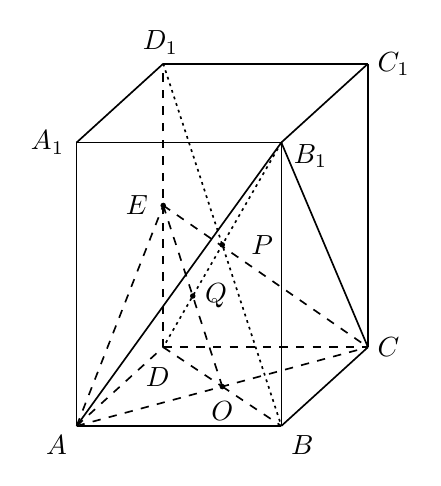
\begin{tikzpicture}[x=1cm,y=1cm,line width=.6pt,font=\normalsize]
\tikzset{ptlabel/.style={font=\normalsize,inner sep=1.2pt}}
% Straight square prism ABCD-A1B1C1D1, E midpoint of D1D; rich interior construction
\coordinate (A) at (0,0);
\coordinate (B) at (2.6,0);
\coordinate (C) at (3.7,1.0);
\coordinate (D) at (1.1,1.0);
\coordinate (A1) at (0,3.6);
\coordinate (B1) at (2.6,3.6);
\coordinate (C1) at (3.7,4.6);
\coordinate (D1) at (1.1,4.6);
\coordinate (E) at (1.1,2.8);
\coordinate (O) at (1.85,0.5);
% outer solid
\draw (A) -- (B);
\draw (B) -- (C);
\draw (B) -- (B1);
\draw (C) -- (C1);
\draw (A) -- (A1);
\draw (A1) -- (B1);
\draw (B1) -- (C1);
\draw (C1) -- (D1);
\draw (D1) -- (A1);
% bold solid diagonals of front/right faces (match noisy original)
\draw (A) -- (B1);
\draw (B1) -- (C);
% hidden base dashed
\draw[dashed] (A) -- (D);
\draw[dashed] (D) -- (C);


\draw[dashed] (D) -- (O);
\draw[dashed] (O) -- (B);
\draw[dashed] (D) -- (D1);

% triangle EAC dashed
\draw[dashed] (A) -- (E);
\draw[dashed] (E) -- (C);
\draw[dashed] (A) -- (C);
% D1B and B1D dotted->dashed (original dotted scan)
\draw[dashed,dash pattern=on 1pt off 1.5pt] (D1) -- (B);
\draw[dashed,dash pattern=on 1pt off 1.5pt] (B1) -- (D);
% EO dashed
\draw[dashed] (E) -- (O);
% P,Q on B1D segment (schematic positions along B1-D)
\coordinate (P) at (1.8500000000,2.3000000000);
\coordinate (Q) at (1.4750000000,1.6500000000);
\fill (P) circle (1pt);
\fill (Q) circle (1pt);
\fill (E) circle (1pt);
\fill (O) circle (1pt);
% labels
\node[ptlabel,below left,xshift=-2pt,yshift=-2pt] at (A) {$A$};
\node[ptlabel,below right,xshift=2pt,yshift=-2pt] at (B) {$B$};
\node[ptlabel,right,xshift=2pt] at (C) {$C$};
\node[ptlabel,below,xshift=-2pt,yshift=-6pt] at (D) {$D$};
\node[ptlabel,left,xshift=-3pt] at (A1) {$A_{1}$};
\node[ptlabel,right,xshift=3pt,yshift=-5pt] at (B1) {$B_{1}$};
\node[ptlabel,right,xshift=2pt] at (C1) {$C_{1}$};
\node[ptlabel,above,xshift=-1pt,yshift=2pt] at (D1) {$D_{1}$};
\node[ptlabel,left,xshift=-4pt] at (E) {$E$};
\node[ptlabel,below,yshift=-4pt] at (O) {$O$};
\node[ptlabel,right,xshift=9pt] at (P) {$P$};
\node[ptlabel,right,xshift=3pt] at (Q) {$Q$};
\end{tikzpicture}
